\documentclass[tikz,border=12pt]{standalone}
\usepackage{amsmath,amssymb,amsfonts}
\usepackage{tikz}
\usetikzlibrary{shapes,arrows.meta,positioning,calc,fit,backgrounds,decorations.pathreplacing,shadows}

% --- Color Palette ---
\definecolor{themeblue}{RGB}{37, 99, 235}
\definecolor{themeteal}{RGB}{13, 148, 136}
\definecolor{themepurple}{RGB}{124, 58, 237}
\definecolor{themeorange}{RGB}{234, 88, 12}
\definecolor{themegreen}{RGB}{22, 163, 74}
\definecolor{themered}{RGB}{220, 38, 38}
\definecolor{themegray}{RGB}{100, 116, 139}
\definecolor{themecyan}{RGB}{6, 182, 212}
\definecolor{themeamber}{RGB}{217, 119, 6}

\begin{document}
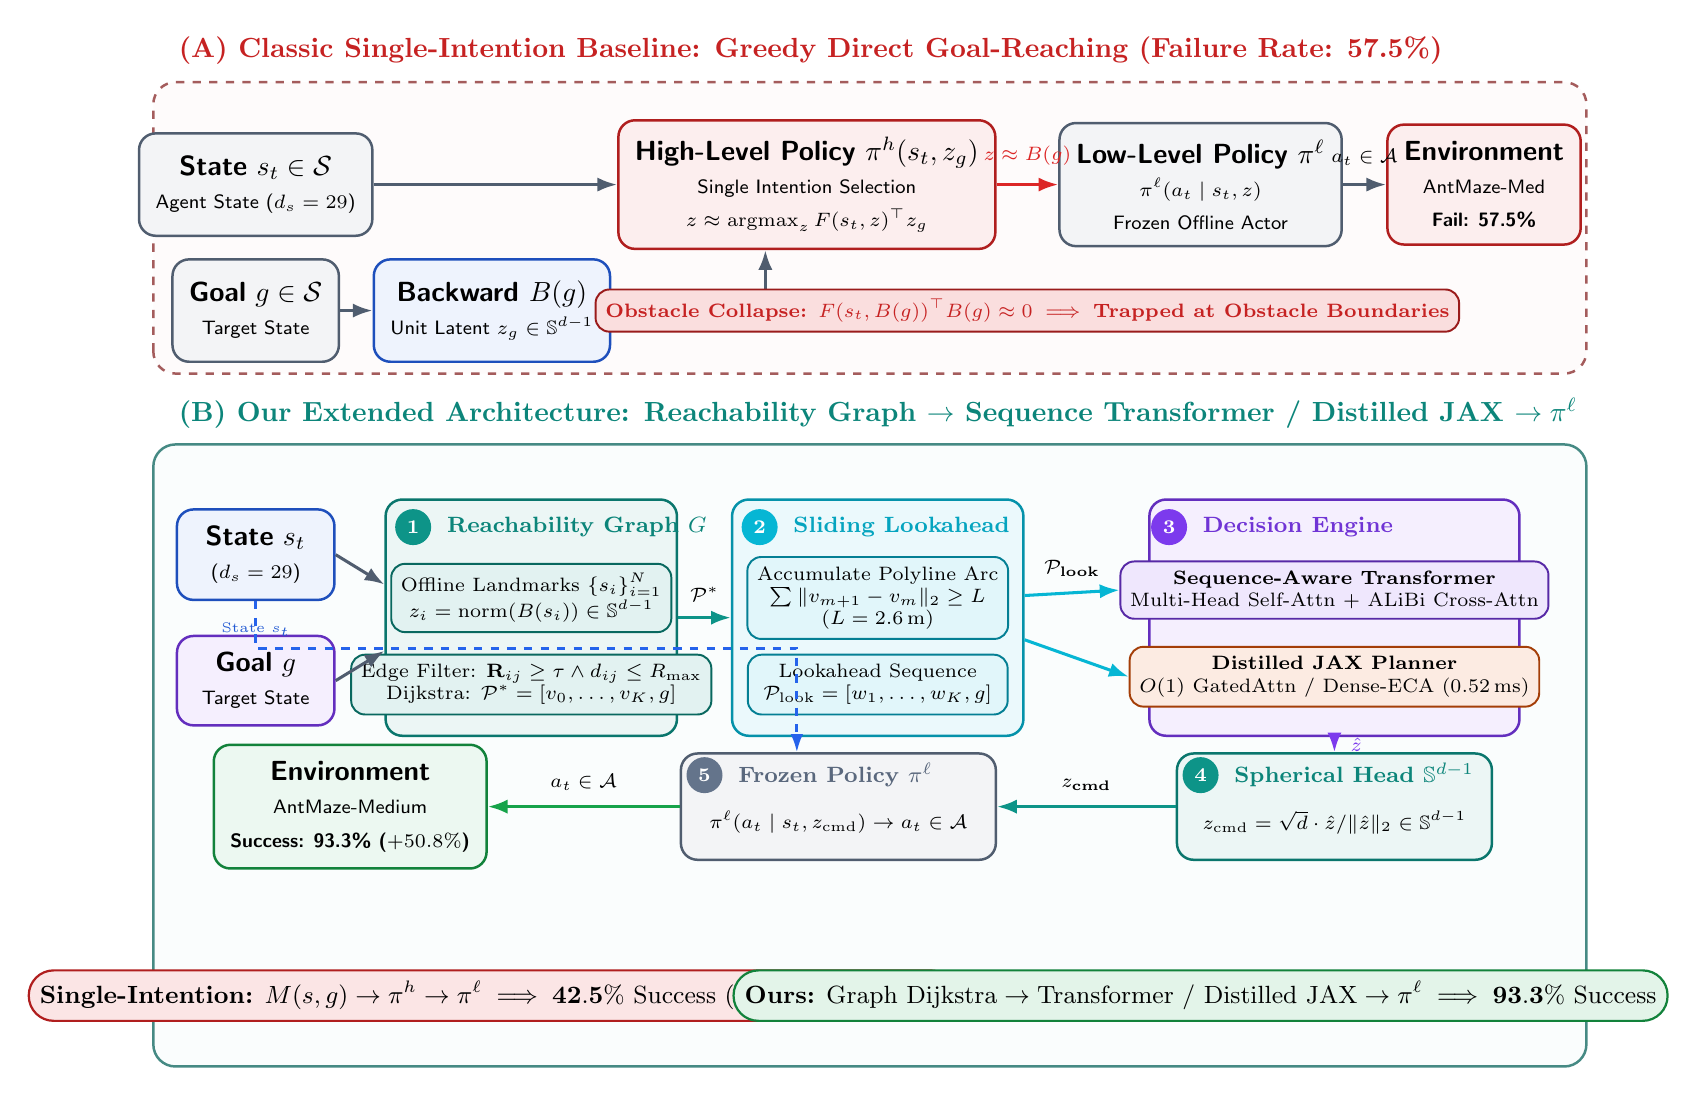
\begin{tikzpicture}[
    >=Latex,
    font=\sffamily,
    % Node styles
    box/.style={
        rectangle,
        rounded corners=6pt,
        draw=#1!80!black,
        fill=#1!8,
        line width=0.9pt,
        align=center,
        inner sep=6pt
    },
    subbox/.style={
        rectangle,
        rounded corners=5pt,
        draw=#1!70!black,
        fill=#1!12,
        line width=0.7pt,
        align=center,
        inner sep=3.5pt
    },
    badge/.style={
        circle,
        fill=#1,
        text=white,
        font=\bfseries\scriptsize,
        inner sep=0.5pt,
        minimum size=13pt
    },
    pill/.style={
        rectangle,
        rounded corners=9pt,
        draw=#1!80!black,
        fill=#1!12,
        line width=0.8pt,
        align=center,
        inner sep=4pt
    },
    arr/.style={
        -{Latex[length=2.5mm,width=1.8mm]},
        line width=1.1pt,
        draw=themegray!80!black
    },
    carr/.style={
        -{Latex[length=2.5mm,width=1.8mm]},
        line width=1.1pt,
        draw=#1
    },
    darr/.style={
        -{Latex[length=2.3mm,width=1.6mm]},
        line width=1.0pt,
        dashed,
        draw=#1
    }
]

% ==============================================================================
% TOP PANEL: (A) Single-Intention Baseline
% ==============================================================================
\node[anchor=west, font=\bfseries\normalsize, text=themered!90!black] at (-0.3, 8.4) 
    {(A) Classic Single-Intention Baseline: Greedy Direct Goal-Reaching (Failure Rate: 57.5\%)};

% Baseline Enclosing Box
\draw[rounded corners=8pt, line width=0.9pt, draw=themered!40!gray, fill=themered!2, dashed] 
    (-0.5, 4.3) rectangle (17.7, 8.0);

% Baseline Nodes
\node[box=themegray, minimum width=2.1cm, minimum height=1.3cm] (b_s) at (0.8, 6.7) 
    {\textbf{State} $s_t \in \mathcal{S}$\\\scriptsize Agent State ($d_s=29$)};

\node[box=themegray, minimum width=2.1cm, minimum height=1.3cm] (b_g) at (0.8, 5.1) 
    {\textbf{Goal} $g \in \mathcal{S}$\\\scriptsize Target State};

\node[box=themeblue, minimum width=2.4cm, minimum height=1.3cm] (b_bg) at (3.8, 5.1) 
    {\textbf{Backward $B(g)$}\\\scriptsize Unit Latent $z_g \in \mathbb{S}^{d-1}$};

\node[box=themered, minimum width=3.3cm, minimum height=1.5cm] (b_pih) at (7.8, 6.7) 
    {\textbf{High-Level Policy} $\pi^h(s_t, z_g)$\\\scriptsize Single Intention Selection\\\scriptsize $z \approx \operatorname{argmax}_z F(s_t, z)^\top z_g$};

\node[box=themegray, minimum width=2.7cm, minimum height=1.5cm] (b_pil) at (12.8, 6.7) 
    {\textbf{Low-Level Policy} $\pi^\ell$\\\scriptsize $\pi^\ell(a_t \mid s_t, z)$\\\scriptsize Frozen Offline Actor};

\node[box=themered, minimum width=2.1cm, minimum height=1.5cm] (b_env) at (16.4, 6.7) 
    {\textbf{Environment}\\\scriptsize AntMaze-Med\\\scriptsize \textbf{Fail: 57.5\%}};

% Baseline Connections
\draw[arr] (b_g) -- (b_bg);
\draw[arr] (b_s.east) -- (b_pih.west);
\draw[arr] (b_bg.east) -| ([xshift=-15pt]b_pih.south);
\draw[carr=themered] (b_pih) -- node[midway, above=3pt, font=\scriptsize\bfseries, text=themered] {$z \approx B(g)$} (b_pil);
\draw[arr] (b_pil) -- node[midway, above=3pt, font=\scriptsize] {$a_t \in \mathcal{A}$} (b_env);

% Baseline Failure Callout
\node[subbox=themered, fill=themered!15, text=themered!90!black, font=\scriptsize\bfseries, minimum width=7.2cm] at (10.6, 5.1) 
    {Obstacle Collapse: $F(s_t, B(g))^\top B(g) \approx 0 \implies \text{Trapped at Obstacle Boundaries}$};


% ==============================================================================
% BOTTOM PANEL: (B) Our Extended Topological & Distilled Planning Framework
% ==============================================================================
\node[anchor=west, font=\bfseries\normalsize, text=themeteal!90!black] at (-0.3, 3.8) 
    {(B) Our Extended Architecture: Reachability Graph $\to$ Sequence Transformer / Distilled JAX $\to \pi^\ell$};

% Framework Enclosing Box
\draw[rounded corners=8pt, line width=0.9pt, draw=themeteal!50!gray, fill=themeteal!2] 
    (-0.5, -4.5) rectangle (17.7, 3.4);

% Inputs
\node[box=themeblue, minimum width=2.0cm, minimum height=1.1cm] (f_s) at (0.8, 2.0) 
    {\textbf{State} $s_t$\\\scriptsize ($d_s=29$)};

\node[box=themepurple, minimum width=2.0cm, minimum height=1.1cm] (f_g) at (0.8, 0.4) 
    {\textbf{Goal} $g$\\\scriptsize Target State};

% Step 1: Reachability Graph Card
\node[box=themeteal, minimum width=3.7cm, minimum height=3.0cm] (graph_box) at (4.3, 1.2) {};
\node[badge=themeteal] (b1) at (2.8, 2.35) {1};
\node[font=\bfseries\footnotesize, text=themeteal!90!black, right=2pt of b1] {Reachability Graph $G$};
\node[subbox=themeteal, font=\scriptsize, align=center, minimum width=3.3cm] at (4.3, 1.45) 
    {Offline Landmarks $\{s_i\}_{i=1}^N$\\$z_i = \operatorname{norm}(B(s_i)) \in \mathbb{S}^{d-1}$};
\node[subbox=themeteal, font=\scriptsize, align=center, minimum width=3.3cm] at (4.3, 0.35) 
    {Edge Filter: $\mathbf{R}_{ij} \ge \tau \land d_{ij} \le R_{\max}$\\Dijkstra: $\mathcal{P}^* = [v_0, \dots, v_K, g]$};

% Step 2: Continuous Sliding Lookahead Card
\node[box=themecyan, minimum width=3.7cm, minimum height=3.0cm] (lookahead_box) at (8.7, 1.2) {};
\node[badge=themecyan] (b2) at (7.2, 2.35) {2};
\node[font=\bfseries\footnotesize, text=themecyan!90!black, right=2pt of b2] {Sliding Lookahead};
\node[subbox=themecyan, font=\scriptsize, align=center, minimum width=3.3cm] at (8.7, 1.45) 
    {Accumulate Polyline Arc\\$\sum \|v_{m+1} - v_m\|_2 \ge L$\\($L = 2.6\,\text{m}$)};
\node[subbox=themecyan, font=\scriptsize, align=center, minimum width=3.3cm] at (8.7, 0.35) 
    {Lookahead Sequence\\$\mathcal{P}_{\text{look}} = [w_1, \dots, w_K, g]$};

% Step 3: High-Level Decision Engine Card
\node[box=themepurple, minimum width=4.7cm, minimum height=3.0cm] (engine_box) at (14.5, 1.2) {};
\node[badge=themepurple] (b3) at (12.4, 2.35) {3};
\node[font=\bfseries\footnotesize, text=themepurple!90!black, right=2pt of b3] {Decision Engine};

% Branch A
\node[subbox=themepurple, font=\scriptsize, align=center, minimum width=4.3cm] (branch_a) at (14.5, 1.55) 
    {\textbf{Sequence-Aware Transformer}\\Multi-Head Self-Attn + ALiBi Cross-Attn};

% Branch B
\node[subbox=themeorange, font=\scriptsize, align=center, minimum width=4.3cm] (branch_b) at (14.5, 0.45) 
    {\textbf{Distilled JAX Planner}\\$O(1)$ GatedAttn / Dense-ECA ($0.52\,\text{ms}$)};

% Step 4: Spherical Projection Card
\node[box=themeteal, minimum width=4.0cm, minimum height=1.35cm] (sphere_box) at (14.5, -1.2) {};
\node[badge=themeteal] (b4) at (12.8, -0.8) {4};
\node[font=\bfseries\footnotesize, text=themeteal!90!black, right=2pt of b4] {Spherical Head $\mathbb{S}^{d-1}$};
\node[font=\scriptsize, align=center] at (14.5, -1.4) {$z_{\text{cmd}} = \sqrt{d} \cdot \hat{z} / \|\hat{z}\|_2 \in \mathbb{S}^{d-1}$};

% Step 5: Low-Level Policy Card
\node[box=themegray, minimum width=4.0cm, minimum height=1.35cm] (f_pil) at (8.2, -1.2) {};
\node[badge=themegray] (b5) at (6.5, -0.8) {5};
\node[font=\bfseries\footnotesize, text=themegray!90!black, right=2pt of b5] {Frozen Policy $\pi^\ell$};
\node[font=\scriptsize, align=center] at (8.2, -1.4) {$\pi^\ell(a_t \mid s_t, z_{\text{cmd}}) \to a_t \in \mathcal{A}$};

% Environment
\node[box=themegreen, minimum width=3.0cm, minimum height=1.35cm] (f_env) at (2.0, -1.2) 
    {\textbf{Environment}\\\scriptsize AntMaze-Medium\\\scriptsize \textbf{Success: 93.3\% ($+50.8\%$)}};

% Arrows in Bottom Panel
\draw[arr] (f_s.east) -- ([yshift=12pt]graph_box.west);
\draw[arr] (f_g.east) -- ([yshift=-12pt]graph_box.west);
\draw[carr=themeteal] (graph_box) -- node[above=2pt, font=\scriptsize\bfseries] {$\mathcal{P}^*$} (lookahead_box);
\draw[carr=themecyan] ([yshift=8pt]lookahead_box.east) -- node[above=2pt, font=\scriptsize\bfseries] {$\mathcal{P}_{\text{look}}$} (branch_a.west);
\draw[carr=themecyan] ([yshift=-8pt]lookahead_box.east) -- (branch_b.west);

\draw[carr=themepurple] (engine_box.south) -- node[right=2pt, font=\scriptsize\bfseries, text=themepurple] {$\hat{z}$} (sphere_box.north);

\draw[carr=themeteal] (sphere_box) -- node[above=2pt, font=\scriptsize\bfseries] {$z_{\text{cmd}}$} (f_pil);
\draw[carr=themegreen] (f_pil) -- node[above=2pt, font=\scriptsize\bfseries] {$a_t \in \mathcal{A}$} (f_env);

% State feedback arrow to policy
\draw[darr=themeblue] (f_s.south) -- ++(0,-0.6) -| ([xshift=-15pt]f_pil.north);
\node[font=\tiny, text=themeblue!90!black, anchor=north] at (0.8, 1.25) {State $s_t$};

% ==============================================================================
% BOTTOM SUMMARY PILLS
% ==============================================================================
\node[pill=themered, font=\small, minimum width=8.2cm] at (3.8, -3.6) 
    {\textbf{Single-Intention:} $M(s, g) \to \pi^h \to \pi^\ell \implies \mathbf{42.5\%}\text{ Success}$ (Obstacle Collapse)};

\node[pill=themegreen, font=\small, minimum width=8.6cm] at (12.8, -3.6) 
    {\textbf{Ours:} $\text{Graph Dijkstra} \to \text{Transformer / Distilled JAX} \to \pi^\ell \implies \mathbf{93.3\%}\text{ Success}$};

\end{tikzpicture}
\end{document}
